% Created 2019-05-14 Tue 09:31
% Intended LaTeX compiler: pdflatex
\documentclass[12pt, a4paper]{article}
\usepackage[utf8]{inputenc}
\usepackage[T1]{fontenc}
\usepackage{graphicx}
\usepackage{grffile}
\usepackage{longtable}
\usepackage{wrapfig}
\usepackage{rotating}
\usepackage[normalem]{ulem}
\usepackage{amsmath}
\usepackage{textcomp}
\usepackage{amssymb}
\usepackage{capt-of}
\usepackage{hyperref}
\usepackage[style=authoryear,natbib]{biblatex}
\setlength\bibitemsep{\baselineskip}
\addbibresource{/Users/guilhermesalome/Dropbox/references.bib}
\usepackage[T1]{fontenc}
\usepackage{lmodern}
\usepackage{amsmath}
\usepackage{mathtools}
\usepackage{multirow}
\usepackage{booktabs}
\usepackage{bbm}
\newcommand\numberthis{\addtocounter{equation}{1}\tag{\theequation}}
\newcommand{\E}[1]{\mathbb{E}{\left[#1\right]}}
\newcommand{\EQ}[1]{\mathbb{E}_t^{\mathbb{Q}}{\left[#1\right]}}
\newcommand{\EP}[1]{\mathbb{E}_t^{\mathbb{P}}{\left[#1\right]}}
\newcommand{\e}[1]{\text{e}^{#1}}
\newcommand{\abs}[1]{\left\vert{#1}\right\vert}
\newcommand{\dis}{\overset{d}{\sim}}
\newcommand{\Var}[1]{\mathrm{Var}\left(#1\right)}
\newcommand{\Corr}[1]{\mathrm{Corr}\left(#1\right)}
\newcommand{\Normal}[1]{\mathcal{N}\left(0, #1\right)}
\newcommand{\Max}[1]{\text{max}\left\{#1\right\}}
\newcommand{\Set}[1]{\left\{#1\right\}}
\renewcommand{\ln}[1]{\text{ln}\left(#1\right)}
\DeclareMathOperator*{\argmin}{\arg\!\min}
\DeclareMathOperator*{\argmax}{\arg\!\max}
\DeclarePairedDelimiter\ceil{\lceil}{\rceil}
\DeclarePairedDelimiter\floor{\lfloor}{\rfloor}
\newcommand{\Poisson}[1]{\text{Poisson}\left(#1\right)}
\newcommand{\Uniform}[1]{\text{Unif}#1}
\newcommand{\Cov}[1]{\mathrm{Cov}\left(#1\right)}
\newtheorem{problem}{Problem}
\usepackage[hang,small,bf]{caption}
\usepackage[margin=1in]{geometry}
\usepackage{mathtools}
\usepackage{xcolor}
\usepackage{resizegather}
\usepackage{multirow}
\definecolor{darkgreen}{rgb}{0.1, 0.6, 0.1}
\usepackage{float}
\usepackage{fancyhdr}
\pagestyle{fancy}
\fancypagestyle{plain}{}
\fancyhf{}
\rfoot{Page \thepage}
\usepackage{ifthen}
\rhead{\ifthenelse{\value{page}=1}{Guilherme Salom\'{e}}{Summer \the\year}}
\lhead{\ifthenelse{\value{page}=1}{Econ890-01 Matlab}{Econ890-01 Matlab}}
\usepackage[numbered,framed]{matlab-prettifier}
\usepackage{listings}
\date{}
\title{Plotting}
\hypersetup{
 pdfauthor={Guilherme Salomé},
 pdftitle={Plotting},
 pdfkeywords={},
 pdfsubject={},
 pdfcreator={Emacs 26.1 (Org mode 9.2.1)},
 pdflang={English}}
\begin{document}

\maketitle
Load the housing data set from the last lecture (available \href{https://raw.githubusercontent.com/Salompas/handson-ml/master/datasets/housing/housing.csv}{here}):
\lstset{language=matlab,label= ,caption= ,captionpos=b,firstnumber=1,numbers=left,style=Matlab-editor}
\begin{lstlisting}
% either load the source original data: readtable('housing.csv')
% or the version we cleaned
load('housing_clean.mat');
data = data_no_missing;
clear data_no_missing;
\end{lstlisting}
\section{Histogram}
\label{sec:org6d2af92}
\begin{figure}[H]
\centering
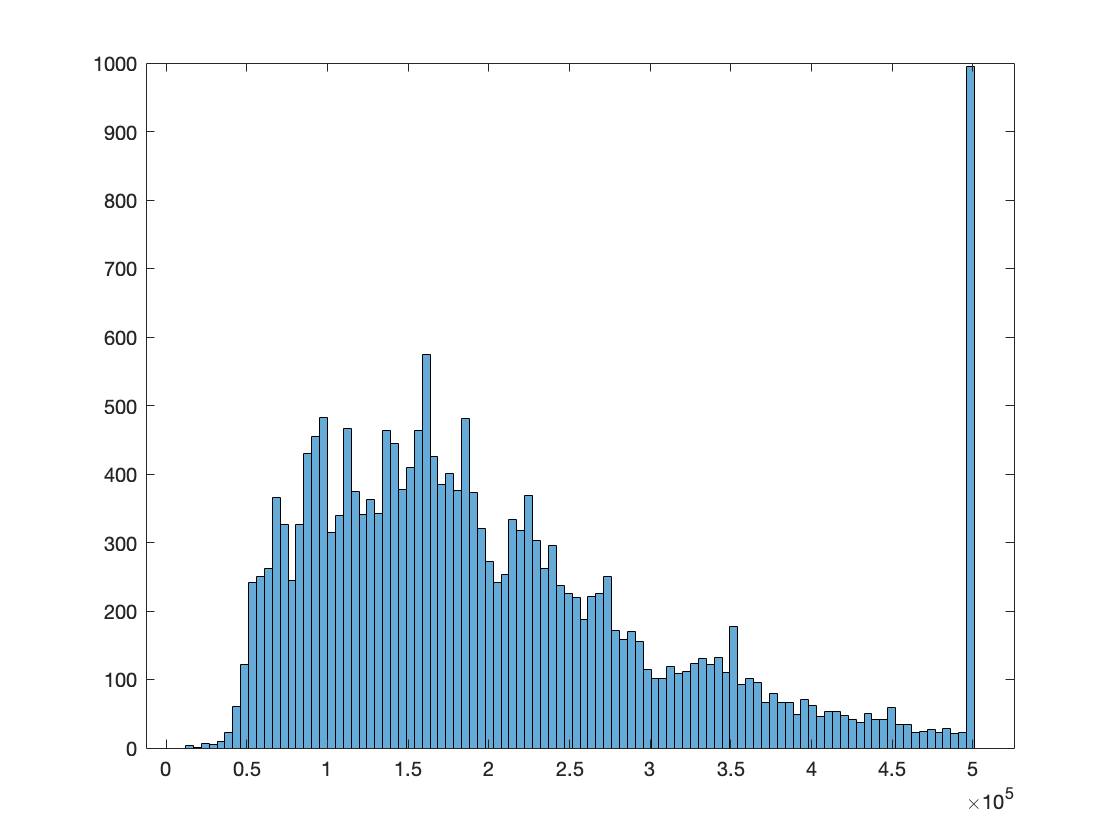
\includegraphics[width=8cm]{/Users/guilhermesalome/Teaching/Duke/Econ890 Matlab - 2019/supporting/matlab_histogram.png}
\caption{\label{fig:orgc3e358e}
A Simple Histogram.}
\end{figure}

We can better understand a data set by creating histograms of its variables.
In Matlab, the function \href{https://www.mathworks.com/help/matlab/ref/matlab.graphics.chart.primitive.histogram.html}{\texttt{histogram}} can generate histograms and has several configurable properties:
\lstset{language=matlab,label= ,caption= ,captionpos=b,firstnumber=1,numbers=left,style=Matlab-editor}
\begin{lstlisting}
% create a histogram for median_house_value
histogram(data.median_house_value);
% histogram automatically determines number of bins and widths
% but we can define it ourselves
histogram(data.median_house_value, 100); % 100 bins
% histogram also works with categorical data
\end{lstlisting}
We can also create histograms for categorical data.
We can create a categorical array from another array with the \href{https://www.mathworks.com/help/matlab/ref/categorical.html}{\texttt{categorical}} function, which can then be used to create a histogram.
\lstset{language=matlab,label= ,caption= ,captionpos=b,firstnumber=1,numbers=left,style=Matlab-editor}
\begin{lstlisting}
% convert string array to categorical data
ocean_proximity = categorical(data.ocean_proximity);
histogram(ocean_proximity);
\end{lstlisting}
\section{Scatter Plot}
\label{sec:org716b43a}
\begin{figure}[H]
\centering
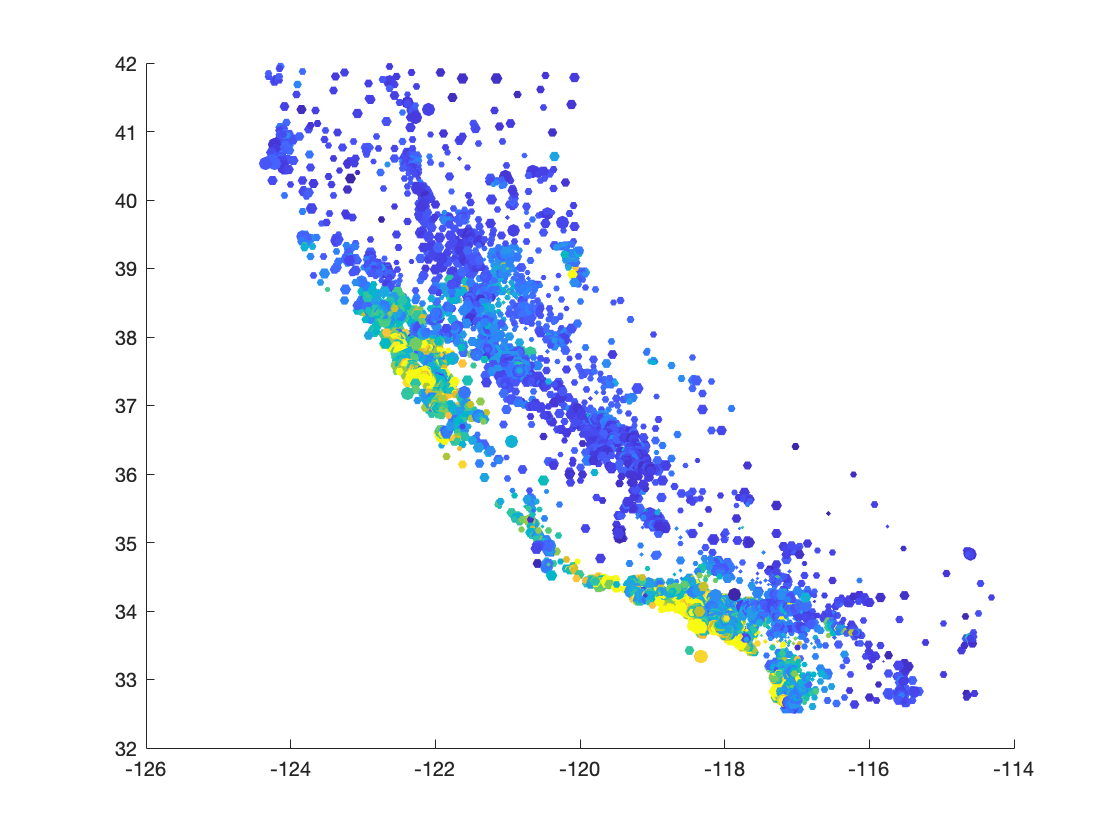
\includegraphics[width=8cm]{/Users/guilhermesalome/Teaching/Duke/Econ890 Matlab - 2019/supporting/matlab_scatter_plot.png}
\caption{\label{fig:orgab460eb}
A Simple Scatter Plot.}
\end{figure}

To create a scatter plot we use the \href{https://www.mathworks.com/help/matlab/ref/scatter.html}{\texttt{scatter}} function.
\lstset{language=matlab,label= ,caption= ,captionpos=b,firstnumber=1,numbers=left,style=Matlab-editor}
\begin{lstlisting}
% scatter takes 2 main arguments: x and y values
scatter(data.longitude, data.latitude)
% we can change the shape, size and color of the points
% syntax: size, color, symbol
scatter(data.longitude, data.latitude, '+')
scatter(data.longitude, data.latitude, '.')
scatter(data.longitude, data.latitude, 2, '.')
scatter(data.longitude, data.latitude, 200, '.')
scatter(data.longitude, data.latitude, 2, 'black', '.')
% we can use another variable to determine the size of the points
scatter(data.longitude, data.latitude, data.median_house_value./1000, ...
        'black', 'o', 'filled');
% the filled option fills in the circles
% we can use another variable to determine the color of the points
scatter(data.longitude, data.latitude, 2, data.median_house_value./1000, '.');
colorbar; % add a colorbar to the figure
% we can do both
scatter(data.longitude, data.latitude, 10*data.housing_median_age, ...
        data.median_house_value./1000, '.');
\end{lstlisting}
Matlab accepts color definitions in \href{https://www.mathworks.com/help/matlab/ref/colorspec.html}{three ways}: RGB values, short names or long names.
RGB values are defined as vectors with three numbers, each defining how much red, green and blue should be displayed.
The short names are shortcuts for the color long names, and a full list of the color names is available \href{https://www.mathworks.com/help/matlab/ref/colorspec.html}{here}.
A complete list of the properties of a figure is available \href{https://www.mathworks.com/help/matlab/ref/matlab.ui.figure-properties.html}{here}.
\section{Specifying Labels, Legends and Title}
\label{sec:orgeefb934}
\begin{figure}[H]
\centering
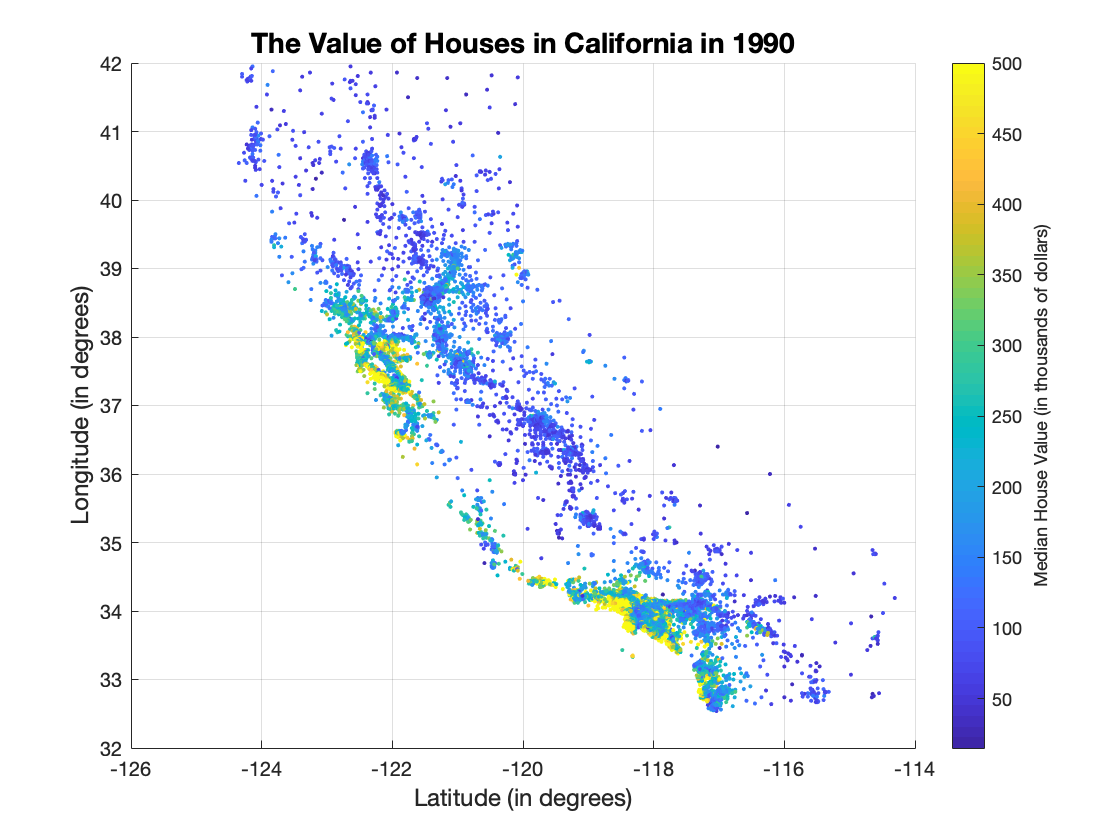
\includegraphics[width=8cm]{/Users/guilhermesalome/Teaching/Duke/Econ890 Matlab - 2019/supporting/matlab_specifying_labels.png}
\caption{\label{fig:org8b9713a}
Specifying Labels, Legends and Title.}
\end{figure}

There are several functions to specify labels, legends and the title of a figure.
\lstset{language=matlab,label= ,caption= ,captionpos=b,firstnumber=1,numbers=left,style=Matlab-editor}
\begin{lstlisting}
% create scatter plot with color varying with house value
scatter(data.longitude, data.latitude, 20, data.median_house_value./1000, ...
        '.');
% add labels
xlabel('Latitude (in degrees)');
ylabel('Longitude (in degrees)');
% change font size of labels
xlabel('Latitude (in degrees)', 'FontSize', 12);
ylabel('Longitude (in degrees)', 'FontSize', 12);
% add a title
title('The Value of Houses in California in 1990', 'FontSize', 14);
% add a grid to the plot
grid on;
% add colorbar
cbar = colorbar;
cbar.Label.String = 'Median House Value (in thousands of dollars)';
cbar.Label.FontSize = 12;
\end{lstlisting}
Links to the documentation for the functions used above: \href{https://www.mathworks.com/help/matlab/ref/xlabel.html}{\texttt{xlabel}}, \href{https://www.mathworks.com/help/matlab/ref/ylabel.html}{\texttt{ylabel}}, \href{https://www.mathworks.com/help/matlab/ref/title.html?s\_tid=doc\_ta}{\texttt{title}}, \href{https://www.mathworks.com/help/matlab/ref/grid.html}{\texttt{grid}} and \href{https://www.mathworks.com/help/matlab/ref/colorbar.html}{\texttt{colorbar}}.
\section{Saving a Figure}
\label{sec:org8e097f0}
We can save a figure to a \texttt{.fig} file with the function \href{https://www.mathworks.com/help/matlab/ref/savefig.html?s\_tid=doc\_ta}{\texttt{savefig}}, which is similar to a \texttt{.mat} file for variables.
This allows us to reopen the figure in Matlab with the function \href{https://www.mathworks.com/help/matlab/ref/openfig.html}{\texttt{openfig}}.
\lstset{language=matlab,label= ,caption= ,captionpos=b,firstnumber=1,numbers=left,style=Matlab-editor}
\begin{lstlisting}
% save figure to .fig file
savefig('house_value');
savefig('house_value.fig'); % equivalent
% close the figure by closing the window
% reload it
openfig('house_value.fig');
\end{lstlisting}
We can also save a figure to a file that can opened by other software, like \texttt{.png} files.
This can be done with the function \href{https://www.mathworks.com/help/matlab/ref/print.html}{\texttt{print}}:
\lstset{language=matlab,label= ,caption= ,captionpos=b,firstnumber=1,numbers=left,style=Matlab-editor}
\begin{lstlisting}
% save figure as .png
print('house_value', '-dpng');
% save figure as .jpg
print('house_value', '-djpeg');
% save figure as .png with a resolution of 300 dots per inch
print('house_value', '-dpng', '-r300');
\end{lstlisting}
\section{2-D Line Plot}
\label{sec:org90f17f8}
\begin{figure}[H]
\centering
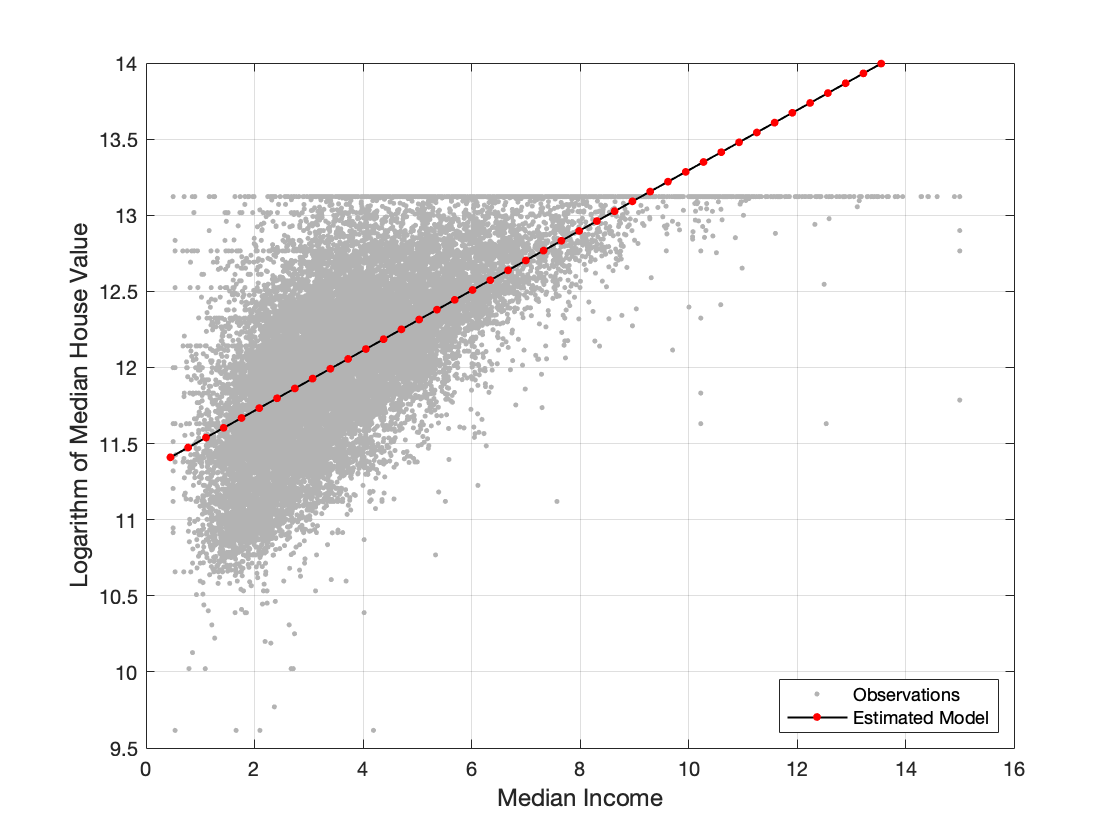
\includegraphics[width=8cm]{/Users/guilhermesalome/Teaching/Duke/Econ890 Matlab - 2019/supporting/matlab_2d_line_plots.png}
\caption{\label{fig:org86ca9fb}
2-D Line Plots.}
\end{figure}

Let's create a line plot representing the result of a linear regression using the function \href{https://www.mathworks.com/help/matlab/ref/plot.html}{\texttt{plot}}:
\lstset{language=matlab,label= ,caption= ,captionpos=b,firstnumber=1,numbers=left,style=Matlab-editor}
\begin{lstlisting}
% regression of logarithm of median house value on median income
result = linreg_ols(log(data.median_house_value), data.median_income);
% 2D-plot of the estimated regression
% define range of values
x_min = 0.9*min(data.median_income);
x_max = 1.1*max(data.median_income);
% generate 50 points between x_min and x_max
x = linspace(x_min, x_max, 50);
y = result.b(1) + result.b(2)*x;
% actual plot
plot(x, y);
% change the line style
plot(x, y, 'LineStyle', '--');
% other values '-' (default), ':', ':.'
% mark the data points in the line with an x
plot(x, y, 'Marker', 'x');
% change marker size
plot(x, y, 'Marker', 'x', 'MarkerSize', 2);
% change the color of the line
plot(x, y, 'Marker', 'x', 'Color', 'black');
% change the width of the line
plot(x, y, 'Color', 'black', 'LineWidth', 1);
% change the color of the marker
plot(x, y, 'Marker', '.', 'MarkerEdgeColor', 'red', 'MarkerSize', 10, ...
     'Color', 'black', 'LineWidth', 1);
\end{lstlisting}
Let's add in a scatter plot containing the original data points.
To add a new plot on an already existing plot, we need to use the command \href{https://www.mathworks.com/help/matlab/ref/hold.html}{\texttt{hold}}.
We can call \texttt{hold on} so that new plot commands are added to the same figure, and then \texttt{hold off} when we want new plot commands to generate new figures.
\lstset{language=matlab,label= ,caption= ,captionpos=b,firstnumber=1,numbers=left,style=Matlab-editor}
\begin{lstlisting}
hold on;
% add a scatter plot with the original data
% save the scatter object so that we can modify the properties
% after the figure is generated
sobj = scatter(data.median_income, log(data.median_house_value));
% let's modify the scatter properties with the scatter object saved
% in the splot variable
sobj.Marker = '.';
sobj.MarkerEdgeColor = [0.7 0.7 0.7];
\end{lstlisting}
Notice that the points of the scatter are on top of the line.
We can change this by code with the function \href{https://www.mathworks.com/help/matlab/ref/uistack.html}{\texttt{uistack}}:
\lstset{language=matlab,label= ,caption= ,captionpos=b,firstnumber=1,numbers=left,style=Matlab-editor}
\begin{lstlisting}
uistack(sobj, 'bottom');
\end{lstlisting}
Alternatively, you would need to recreate the figure and change the order of the plots (first create the scatter, then \texttt{hold on} and create the line plot).

Let's now add a grid to the figure, labels, title and a \href{https://www.mathworks.com/help/matlab/ref/legend.html}{\texttt{legend}}:
\lstset{language=matlab,label= ,caption= ,captionpos=b,firstnumber=1,numbers=left,style=Matlab-editor}
\begin{lstlisting}
% add grid
grid on;
% add labels
xlabel('Median Income', 'FontSize', 12);
ylabel('Logarithm of Median House Value', 'FontSize', 12);
% add a legend for the line plot and for the scatter
% also move the legend location so that the line is entirely visible
legend(["Observations", "Estimated Model"], ...
       'Location', 'southeast');
% we can also change the limits of both axes
xlim([0, 16]);
ylim([9.5, 14]);
\end{lstlisting}
Documentation for: \href{https://www.mathworks.com/help/matlab/ref/xlim.html}{\texttt{xlim}} and \href{https://www.mathworks.com/help/matlab/ref/ylim.html}{\texttt{ylim}}.
\section{Latex in Plots}
\label{sec:orgfed42f5}
\begin{figure}[H]
\centering
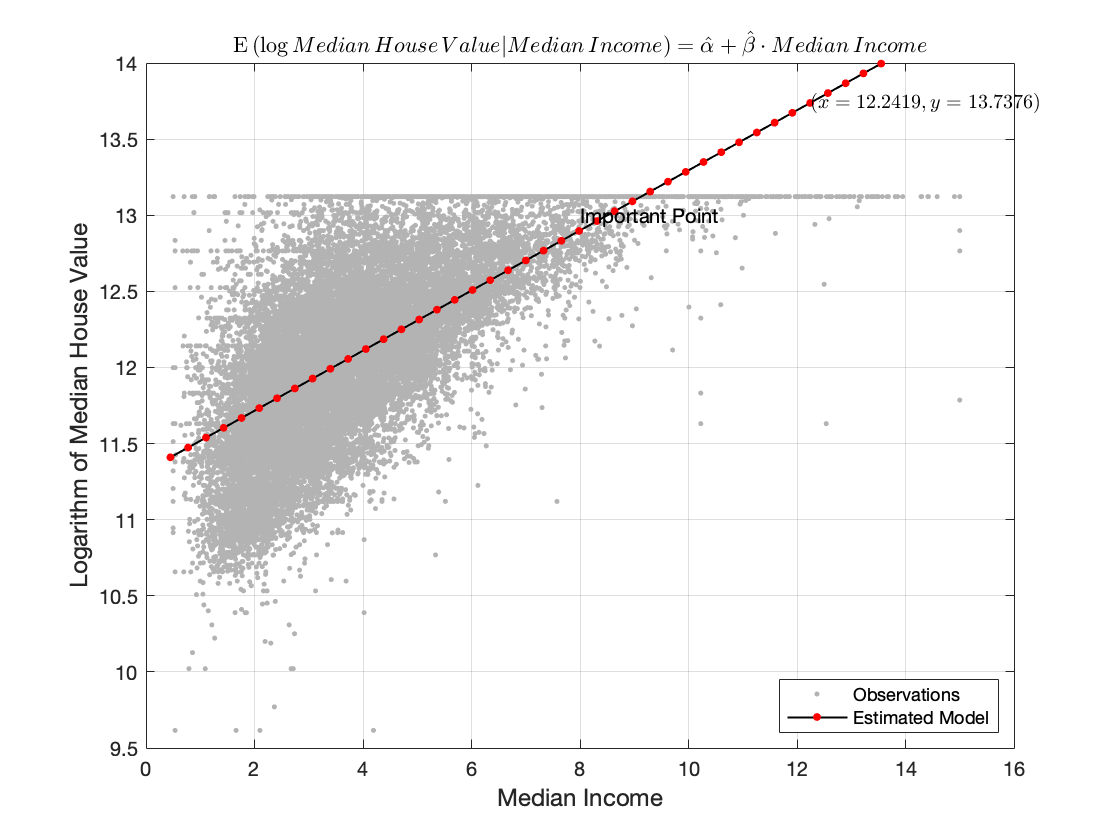
\includegraphics[width=8cm]{/Users/guilhermesalome/Teaching/Duke/Econ890 Matlab - 2019/supporting/matlab_latex_in_plots.png}
\caption{\label{fig:org65cd5f7}
Latex in Plots.}
\end{figure}

Figures in Matlab also support equations created by Latex (to some extent):
\lstset{language=matlab,label= ,caption= ,captionpos=b,firstnumber=1,numbers=left,style=Matlab-editor}
\begin{lstlisting}
title(['$\mathrm{E}\left(\log{Median\, House\, Value\vert Median\, ' ...
       'Income}\right)=\hat{\alpha}+\hat{\beta}\cdot{Median\, ' ...
       'Income}$'], 'Interpreter', 'latex');
\end{lstlisting}
The Latex support is convenient, but is limited to a few basic packages, and extending the number of packages is not straightforward.

We can also add text and Latex equations to the plot itself with the function \href{https://www.mathworks.com/help/matlab/ref/text.html}{\texttt{text}}:
\lstset{language=matlab,label= ,caption= ,captionpos=b,firstnumber=1,numbers=left,style=Matlab-editor}
\begin{lstlisting}
% specify a point in the plot to add the text to
text(8, 13, 'Important Point', 'FontSize', 10);
% latex can also be used
text(12.2419, 13.7376, '$(x=12.2419, y=13.7376)$', 'Interpreter', 'latex');
\end{lstlisting}
\section{Surface Plot}
\label{sec:org644f29d}
\begin{figure}[H]
\centering
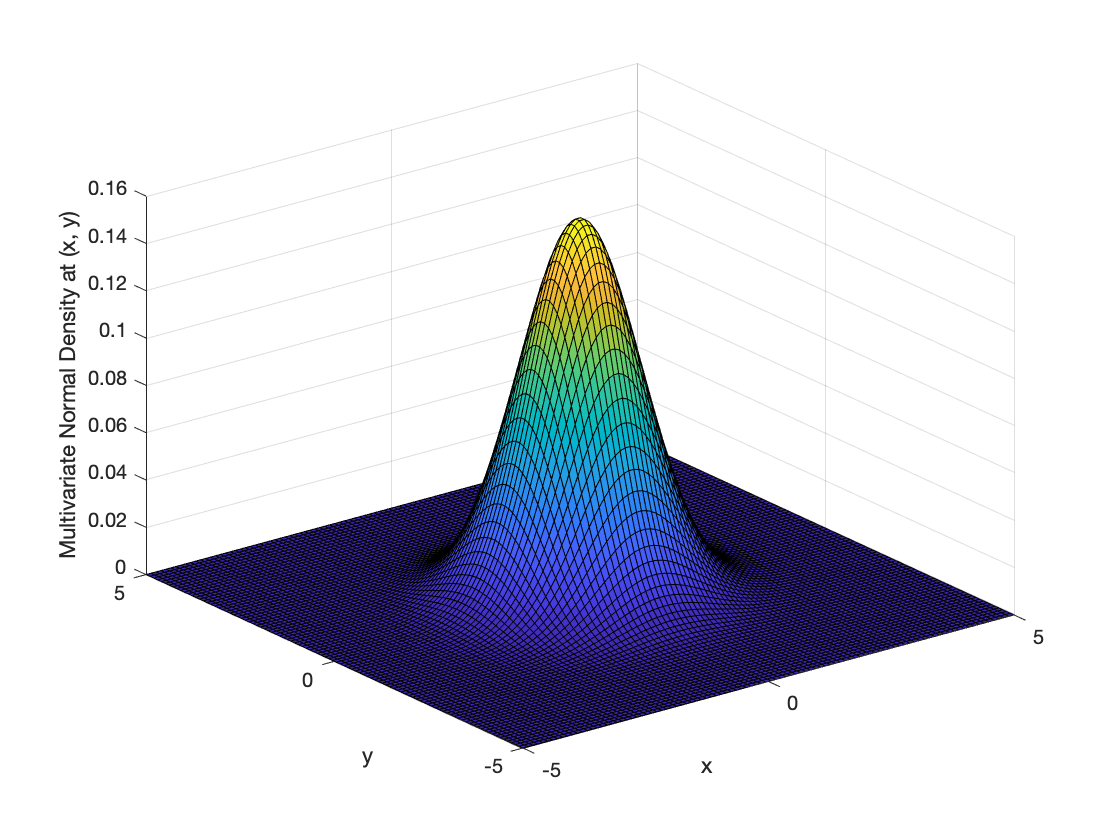
\includegraphics[width=8cm]{/Users/guilhermesalome/Teaching/Duke/Econ890 Matlab - 2019/supporting/matlab_surface_plot.png}
\caption{\label{fig:orgba05dfd}
Surface Plot of a 2-Dimensional Normal Distribution Density.}
\end{figure}

We can create a surface plot with the function \href{https://www.mathworks.com/help/matlab/ref/surf.html}{\texttt{surf}}.
Let's plot the density of a multivariate normal distribution using \href{https://www.mathworks.com/help/stats/mvnpdf.html}{\texttt{mvnpdf}}:
\lstset{language=matlab,label= ,caption= ,captionpos=b,firstnumber=1,numbers=left,style=Matlab-editor}
\begin{lstlisting}
% generate points for the x-axis and for the y-axis
x = linspace(-5, 5);
y = linspace(-5, 5);
% create a "cartesian product" or a grid of the x and y points
[X, Y] = meshgrid(x, y);
% mean and variance of a 2-dimensional normal distribution
mu = [0 0];
sigma = [1, 0; 0, 1];
% obtain the density at the different points
% we need to pass to mvnpdf a 2-dimensional matrix containing the x
% and y points (x points on 1st column, y points on 2nd column)
points = [X(:), Y(:)]; % (:) stacks columns of a matrix
Z = mvnpdf(points, mu, sigma);
% reshape the z values to be a matrix
% reshape works by fixing a column and then filling each row, and
% then moving to the next column ...
z = reshape(Z, length(y), length(x));
% create the surface plot
surfplot = surf(x, y, z);
xlabel('x');
ylabel('y');
zlabel('Multivariate Normal Density at (x, y)');
\end{lstlisting}

There are a few important things to notice in the code above.
First, we needed to create a 2-dimensional grid with the x and y points.
We did it with the function \href{https://www.mathworks.com/help/matlab/ref/meshgrid.html}{\texttt{meshgrid}}.
This function takes two vectors, say \(x\) and \(y\), and outputs two matrices, say \(X\) and \(Y\).
The rows of \(X\) are repetitions of the vector \(x\).
The columns of \(Y\) are repetitions of the vector \(y\).
Taking elements of each matrix at the same position gives an element in the grid created by the vectors \(x\) and \(y\):
\begin{align*}
&x = \begin{bmatrix}
x_1\\
\vdots\\
x_n
\end{bmatrix}
y = \begin{bmatrix}
y_1\\
\vdots\\
y_m
\end{bmatrix}\\
&X= \begin{bmatrix}
x_1 & \cdots & x_n\\
x_1 & \cdots & x_n\\
& \vdots& \\
x_1 & \cdots & x_n
\end{bmatrix}_{m\times n}
Y= \begin{bmatrix}
y_1 & \cdots & y_1\\
y_2 & \cdots & y_2\\
& \vdots & \\
y_m & \cdots & y_m
\end{bmatrix}_{m\times n}
\end{align*}

We use the grid represented by the matrices \(X\) and \(Y\) to obtain the density of a 2-dimensional normal distribution.
We pass various 2-dimensional points to the \texttt{mvnpdf} function as a matrix, which we gave the name of \texttt{points}.
We create this matrix my flattening \(X\) and \(Y\) using the syntax \texttt{X(:)} and \texttt{Y(:)}.
The command \texttt{X(:)} stacks all columns of \(X\).
Thus, the \texttt{points} matrix becomes:
\begin{align*}
\text{points} = \begin{bmatrix}
x_1 & y_1\\
x_1 & y_2\\
\vdots&\vdots\\
x_1 & y_m\\
x_2 & y_1\\
x_2 & y_2\\
\vdots&\vdots\\
x_2 & y_m\\
\vdots&\vdots\\
\end{bmatrix}
\end{align*}
The output of \texttt{mvnpdf} stored in \texttt{Z} needs to be reshaped into a matrix for plotting in 3-dimensions:
\begin{align*}
Z = \begin{bmatrix}
z_{(x_1, y_1)}\\
z_{(x_1, y_2)}\\
\vdots\\
z_{(x_1, y_m)}\\
z_{(x_2, y_1)}\\
z_{(x_2, y_2)}\\
\vdots\\
z_{(x_2, y_m)}\\
\vdots
\end{bmatrix}, z= \begin{bmatrix}
z_{(x_1, y_1)} & z_{(x_2, y_1)} & \cdots & z_{(x_n, y_1)}\\
z_{(x_1, y_2)} & z_{(x_2, y_2)} & \cdots & z_{(x_n, y_2)}\\
&& \vdots\\
z_{(x_1, y_m)} & z_{(x_2, y_m)} & \cdots & z_{(x_n, y_m)}
\end{bmatrix}
\end{align*}
To reshape correctly, the resulting matrix \texttt{z} needs to be of dimension \(m \times n\).
With the matrix \(z\) and the vector \(x\) and \(y\) we can create the surface plot.
\section{Plotting Functions}
\label{sec:org96b6866}
\begin{figure}[H]
\centering
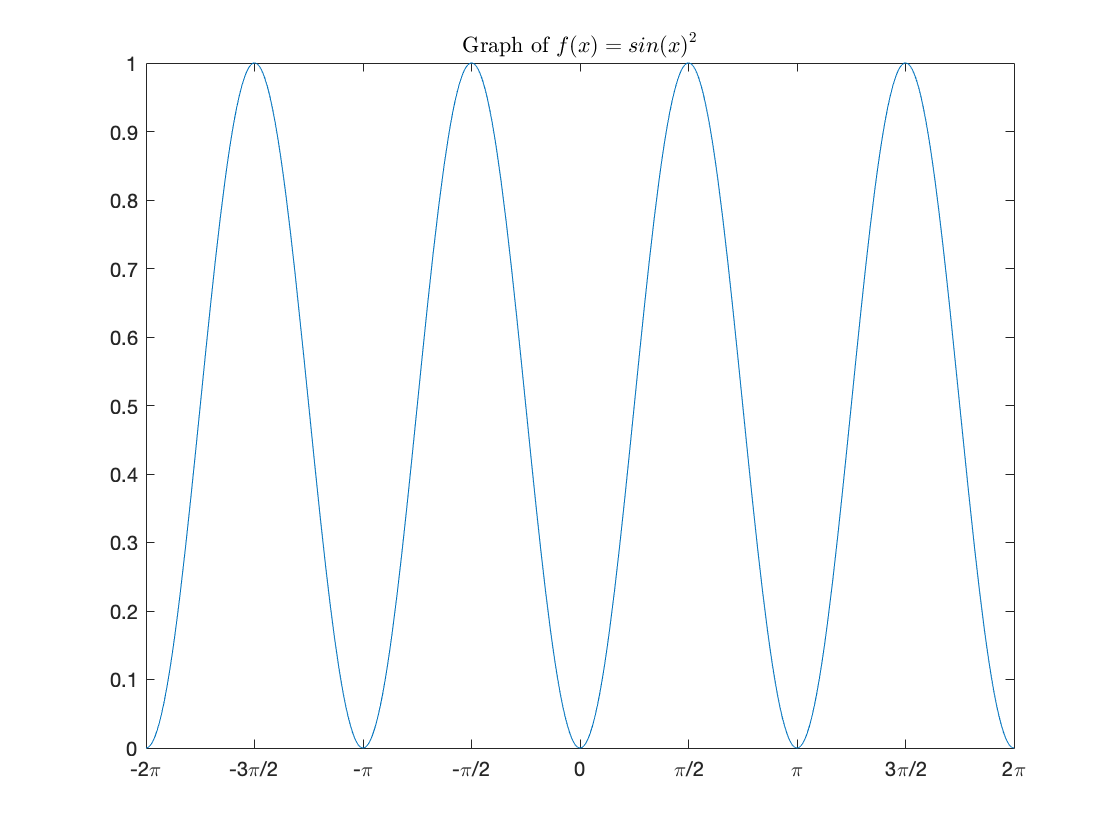
\includegraphics[width=8cm]{/Users/guilhermesalome/Teaching/Duke/Econ890 Matlab - 2019/supporting/matlab_fplot.png}
\caption{\label{fig:orgd64530d}
Plot of a Function.}
\end{figure}

We can quickly plot the graph of a function \(f:\mathbb{R}\mapsto\mathbb{R}\) over some interval using the function \href{https://www.mathworks.com/help/matlab/ref/fplot.html?s\_tid=doc\_ta}{\texttt{fplot}}:
\lstset{language=matlab,label= ,caption= ,captionpos=b,firstnumber=1,numbers=left,style=Matlab-editor}
\begin{lstlisting}
% create a function to plot
f = @(x) sin(x).^2;
% plot the function over some interval
fplot(f, [-2*pi, 2*pi]);
\end{lstlisting}
We can use the functions \href{https://www.mathworks.com/help/matlab/ref/xticks.html?s\_tid=doc\_ta}{\texttt{xticks}} to modify the tick values of the x-axis.
The tick values represent the locations on the x-axis that have the tick marks.
We can then use the function \href{https://www.mathworks.com/help/matlab/ref/xticklabels.html?s\_tid=doc\_ta}{\texttt{xticklabels}} to change the tick labels for the x-axis.
\lstset{language=matlab,label= ,caption= ,captionpos=b,firstnumber=1,numbers=left,style=Matlab-editor}
\begin{lstlisting}
% change the tick values
xticks(-2*pi:pi/2:2*pi);
% change the labels
xticklabels(["-2\pi","-3\pi/2","-\pi","-\pi/2","0","\pi/2","\pi","3\pi/2","2\pi"]);
% add a title
title('Graph of $f(x) = {\sin(x)}^2$', 'Interpreter', 'latex');
\end{lstlisting}
\section{Subplots}
\label{sec:orga0582fd}
\begin{figure}[H]
\centering
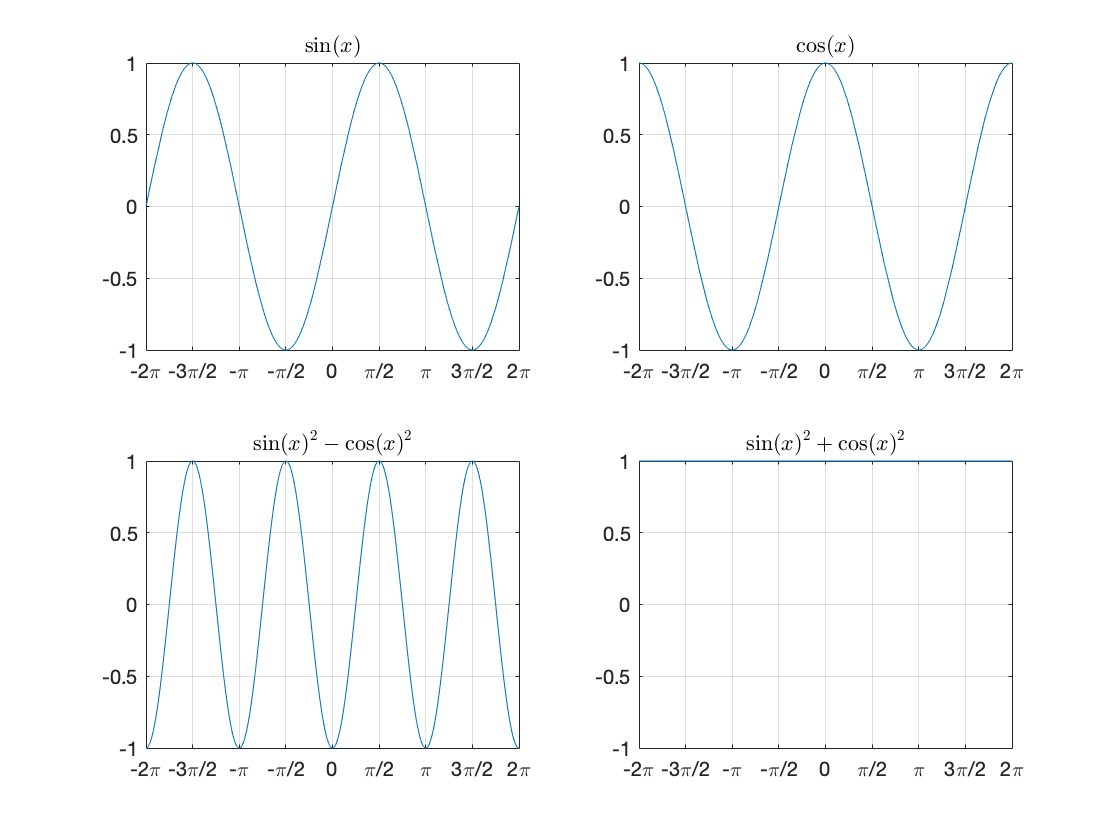
\includegraphics[width=8cm]{/Users/guilhermesalome/Teaching/Duke/Econ890 Matlab - 2019/supporting/matlab_subplots.png}
\caption{\label{fig:org1c31647}
Figure with Multiple Subplots.}
\end{figure}

It is possible to plot multiple figures in a single figure window.
We do so by specifying a grid of subplots, and then we fill each subplot by using the usual plotting commands.
To specify the grid we use the function \href{https://www.mathworks.com/help/matlab/ref/subplot.html?s\_tid=doc\_ta}{\texttt{subplot}}:
\lstset{language=matlab,label= ,caption= ,captionpos=b,firstnumber=1,numbers=left,style=Matlab-editor}
\begin{lstlisting}
% close the previous figure
% create a 2 by 2 grid of subplots and choose the 1st one as the
% current figure to plot on
subplot(2, 2, 1);
% we can now issue plot commands and they will add a figure to the
% first subplot on the 2x2 grid
fplot(@sin, [-2*pi, 2*pi]);
% add labels to the 1st plot
xticks(-2*pi:pi/2:2*pi);
xticklabels(["-2\pi","-3\pi/2","-\pi","-\pi/2","0","\pi/2","\pi","3\pi/2","2\pi"]);
grid on;
title('$\sin(x)$', 'Interpreter', 'latex');

% move the current figure to the 2nd subplot
subplot(2, 2, 2);
% second subplot on the 2x2 grid
fplot(@cos, [-2*pi, 2*pi]);
% add labels to the 2nd plot
xticks(-2*pi:pi/2:2*pi);
xticklabels(["-2\pi","-3\pi/2","-\pi","-\pi/2","0","\pi/2","\pi","3\pi/2","2\pi"]);
grid on;
title('$\cos(x)$', 'Interpreter', 'latex');

% move the current figure to the 3rd subplot
subplot(2, 2, 3);
% third subplot on the 2x2 grid
fplot(@(x) (sin(x).^2 - cos(x).^2), [-2*pi, 2*pi]);
% add labels to the 2nd plot
xticks(-2*pi:pi/2:2*pi);
xticklabels(["-2\pi","-3\pi/2","-\pi","-\pi/2","0","\pi/2","\pi","3\pi/2","2\pi"]);
grid on;
title('${\sin(x)}^2 - {\cos(x)}^2$', 'Interpreter', 'latex');

% move the current figure to the 3rd subplot
subplot(2, 2, 4);
% third subplot on the 2x2 grid
fplot(@(x) (sin(x).^2 + cos(x).^2), [-2*pi, 2*pi]);
% add labels to the 2nd plot
xticks(-2*pi:pi/2:2*pi);
xticklabels(["-2\pi","-3\pi/2","-\pi","-\pi/2","0","\pi/2","\pi","3\pi/2","2\pi"]);
grid on;
title('${\sin(x)}^2 + {\cos(x)}^2$', 'Interpreter', 'latex');
ylim([-1, 1]);
\end{lstlisting}
\section{Default Properties for Plot}
\label{sec:org154891c}
\begin{figure}[H]
\centering
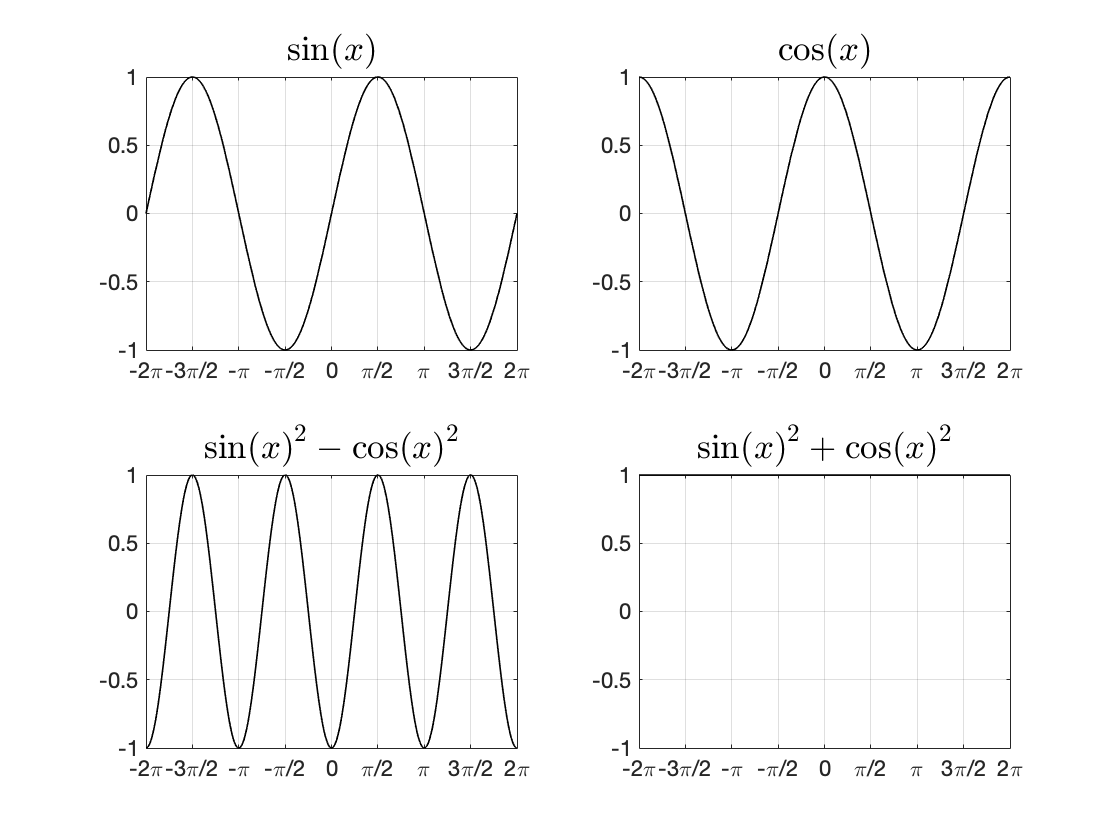
\includegraphics[width=8cm]{/Users/guilhermesalome/Teaching/Duke/Econ890 Matlab - 2019/supporting/matlab_defaults.png}
\caption{\label{fig:org9d9850b}
Figure Created After Setting Plotting Defaults.}
\end{figure}

Several of the properties we modified when plotting can be set up to have different default values, like the size of fonts used, the color and width of plot lines, and so on.
It is useful to have a \texttt{.m} script with all your plotting defaults, and then have this script be run at the beginning of your main program, so that any plots you make have the desired default properties.

\lstset{language=matlab,label= ,caption= ,captionpos=b,firstnumber=1,numbers=left,style=Matlab-editor}
\begin{lstlisting}
% plot_defaults.m
% Changes default values for plots.

% Use Interpreter Latex by Default
% for text
set(groot,'DefaultTextInterpreter','Latex');
% for legends
set(groot,'DefaultLegendInterpreter','Latex');

% Default color order for plots
% Each line is a color defined by an RGB triple
set(groot, 'DefaultAxesColorOrder', [0 0 0; 0.5 0 0; 0 0.5 0; 0 0 0.5]);

% Default line style order
% If we only use one color for plots, then we can cycle through
% line styles
% use only black for plots
set(groot, 'DefaultAxesColorOrder', [0 0 0]);
% but cycle through many styles
set(groot, 'DefaultAxesLineStyleOrder','-|--|:|-.');

% Default line width
def_width = 0.8;
% for line plots
set(groot, 'DefaultLineLineWidth', def_width);
% for scatter plots
set(groot, 'DefaultScatterLineWidth', def_width);
% for function plots
set(groot, 'DefaultFunctionLineLineWidth', def_width);

% Default axes font size (for x-ticks and y-ticks labels)
set(groot,'DefaultAxesFontSize', 12);

% Default title font size
% The font size for the title is defined as a multiplier of the
% font size for the axes
set(groot,'DefaultAxesTitleFontSize', 1.6);

% Default legend font size
set(groot,'DefaultLegendFontSize', 12, ...
          'DefaultLegendFontSizeMode','manual');
\end{lstlisting}
The function \href{https://www.mathworks.com/help/matlab/ref/set.html?s\_tid=doc\_ta}{\texttt{set}} is used to change the properties of the \href{https://www.mathworks.com/help/matlab/ref/groot.html?s\_tid=doc\_ta}{\texttt{groot}} object, which is keeps track of various parameters used by Matlab.
\section{Building Blocks for Figures}
\label{sec:org5193f78}
Matlab offers very good plotting functions that can do the majority of plots we might ever need with few lines of code.
However, to create more complex figures we need to understand some of the building blocks Matlab functions use to create plots.
\subsection{The Figure Window}
\label{sec:orge7396ab}
\begin{figure}[H]
\centering
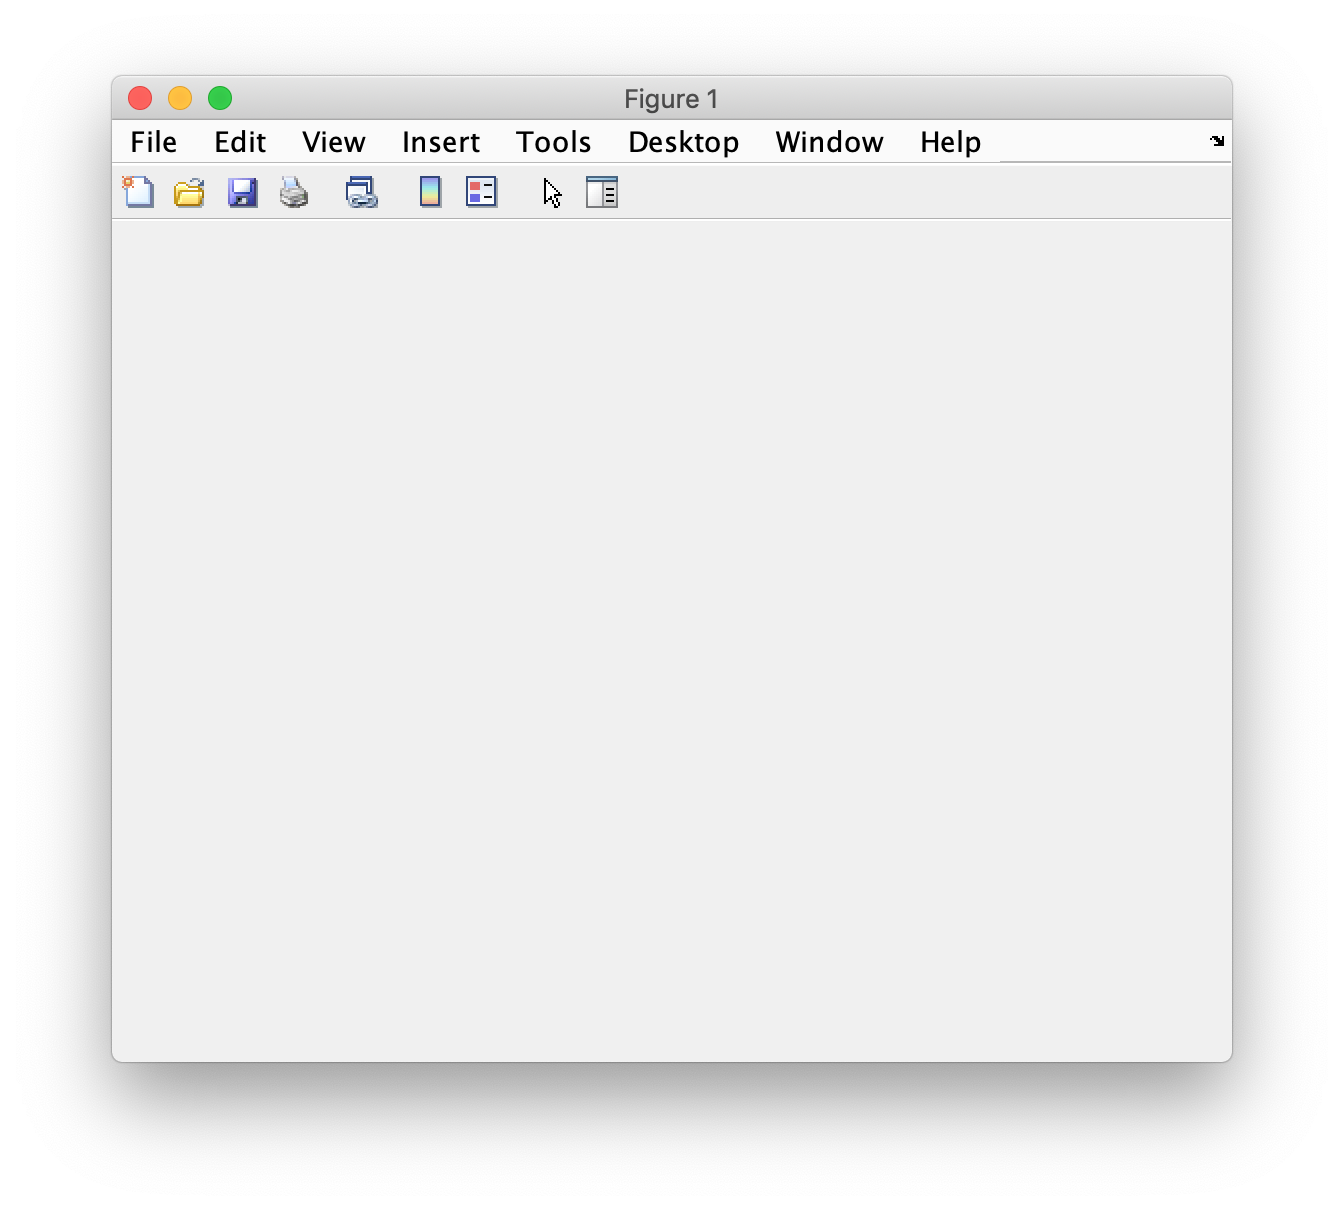
\includegraphics[width=8cm]{/Users/guilhermesalome/Teaching/Duke/Econ890 Matlab - 2019/supporting/matlab_empty_figure_window.png}
\caption{\label{fig:orgc067647}
An Empty Figure Window.}
\end{figure}

The first thing any plotting function does is to tell Matlab to create an empty window to hold the figure.
This window is called the figure window.
When a figure window is created, it becomes the \texttt{current figure} and is the default place where the plotting commands generate the images on this figure.
We can create this figure window with the \href{https://www.mathworks.com/help/matlab/ref/figure.html}{\texttt{figure}} function.
And the handle to the \texttt{current figure} can be accessed via the command \href{https://www.mathworks.com/help/matlab/ref/gcf.html}{\texttt{gcf}}.
\lstset{language=matlab,label= ,caption= ,captionpos=b,firstnumber=1,numbers=left,style=Matlab-editor}
\begin{lstlisting}
figure
\end{lstlisting}
When you run the command above you should see a GUI window pop up.
The window is titled "Figure 1", and it is used to hold plots.
When you close this window, it will \uline{delete} the figure.

When we call \texttt{figure}, it creates returns \texttt{figure object}, which we can assign to a variable.
This is useful to change properties of the figure after its creation.
\lstset{language=matlab,label= ,caption= ,captionpos=b,firstnumber=1,numbers=left,style=Matlab-editor}
\begin{lstlisting}
% assign figure object to variable fig
fig = figure;
% change name of the figure
fig.Name = 'Histogram of Median House Value';
% remove the figure number from the title
fig.NumberTitle = 'off';
% change color
fig.Color = 'Black';
% change color with rgb values
fig.Color = [0.9 0.9 0.9]; % rgb values
% do not display the toolbar
fig.ToolBar = 'none';
% do not display the menu bar
fig.MenuBar = 'none';
% maximize the window
fig.WindowState = 'maximized';
% these properties can be set at the time of creation
close(fig);
fig = figure('Name', 'Histogram of Median House Value', ...
             'NumberTitle', 'off', ...
             'WindowState', 'maximized');
\end{lstlisting}
The \texttt{figure object} is useful to manage several figures windows.
If we have a \texttt{figure object}, we can display its window by calling the function \texttt{figure} passing a figure handle as its input.

The handle to the \texttt{figure object} can also be used to save the figure with \texttt{print}.
\lstset{language=matlab,label= ,caption= ,captionpos=b,firstnumber=1,numbers=left,style=Matlab-editor}
\begin{lstlisting}
fig = figure;
fig.Color = [0.9 0.9 0.9];
print(fig, 'empty_fig', '-dpng', '-r300');
\end{lstlisting}
\subsection{Creating Axes}
\label{sec:org1cfe0bb}
\begin{figure}[H]
\centering
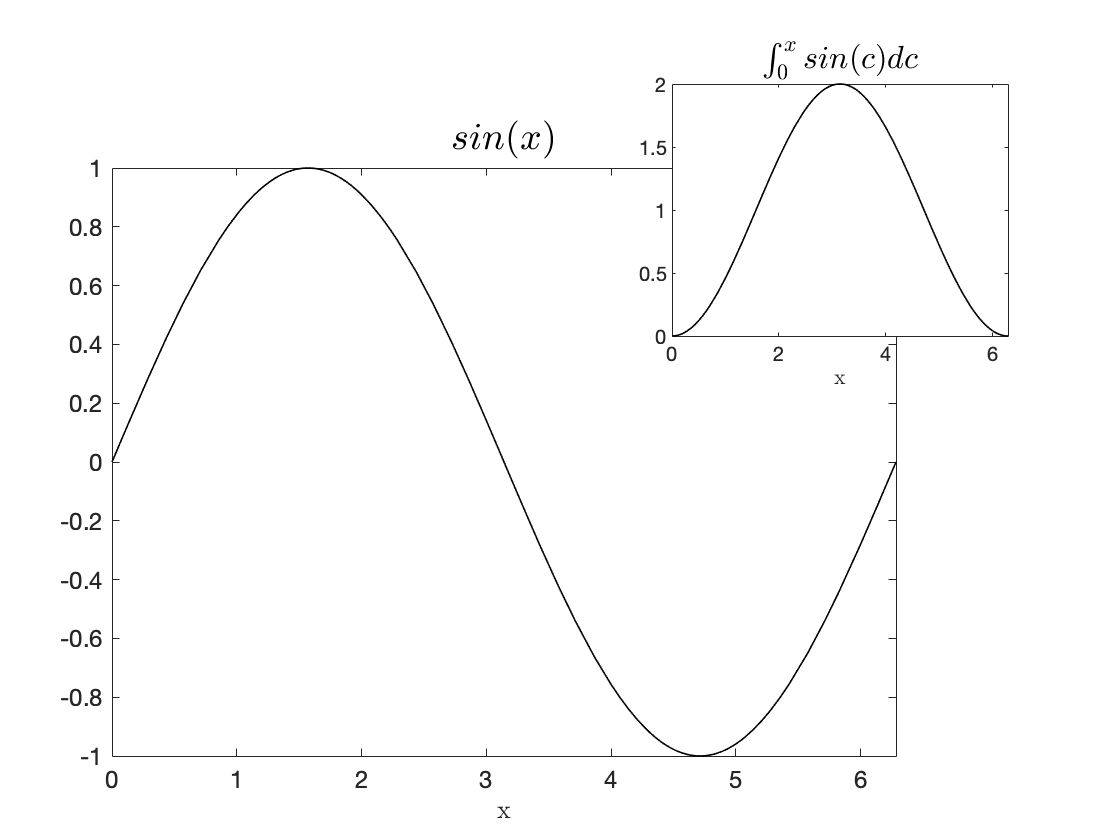
\includegraphics[width=8cm]{/Users/guilhermesalome/Teaching/Duke/Econ890 Matlab - 2019/supporting/matlab_one_figure_two_axes.png}
\caption{\label{fig:org1fd167f}
One Figure with Two Axes.}
\end{figure}

After creating the figure window, we can add axes to it with the function \href{https://www.mathworks.com/help/matlab/ref/axes.html?s\_tid=doc\_ta}{\texttt{axes}}.
We can then plot on these axes and modify their properties to add labels, titles and so on.
\lstset{language=matlab,label= ,caption= ,captionpos=b,firstnumber=1,numbers=left,style=Matlab-editor}
\begin{lstlisting}
% create a figure window
fig = figure;
% add axes to figure
ax1 = axes(fig);
% plot something on the axes
fplot(ax1, @sin, [-2*pi, 2*pi]);
\end{lstlisting}
A single figure can have multiple axes:
\lstset{language=matlab,label= ,caption= ,captionpos=b,firstnumber=1,numbers=left,style=Matlab-editor}
\begin{lstlisting}
% close the previous figure
% create a new figure window
fig = figure;

% add axes to figure specifying its position
ax1 = axes(fig, 'Position', [0.1 0.1 0.7 0.7]);
% the first 2 numbers specify the left and bottom positions of the
% axes in the figure window
% the last 2 numbers specify the width and height of the axes
% we do not use [0 0 0.7 0.7] because we need space for the tick
% labels

% add a 2nd axes that is smaller
ax2 = axes(fig, 'Position', [0.6 0.6 0.3 0.3]);

% plot on ax1
fplot(ax1, @sin, [0, 2*pi]);

% plot on ax2
fplot(ax2, @(x) (integral(@sin, 0, x)), [0, 2*pi]);
\end{lstlisting}
We can add labels and a title to each of the axes:
\lstset{language=matlab,label= ,caption= ,captionpos=b,firstnumber=1,numbers=left,style=Matlab-editor}
\begin{lstlisting}
% add title to axes
ax1.Title.String = '$sin(x)$';
ax2.Title.String = '$\int_0^x sin(c)dc$';

% add labels to axes
ax1.XLabel.String = 'x';
ax2.XLabel.String = 'x';
\end{lstlisting}
\subsection{Manipulating Axes}
\label{sec:org19bfa40}
\begin{figure}[H]
\centering
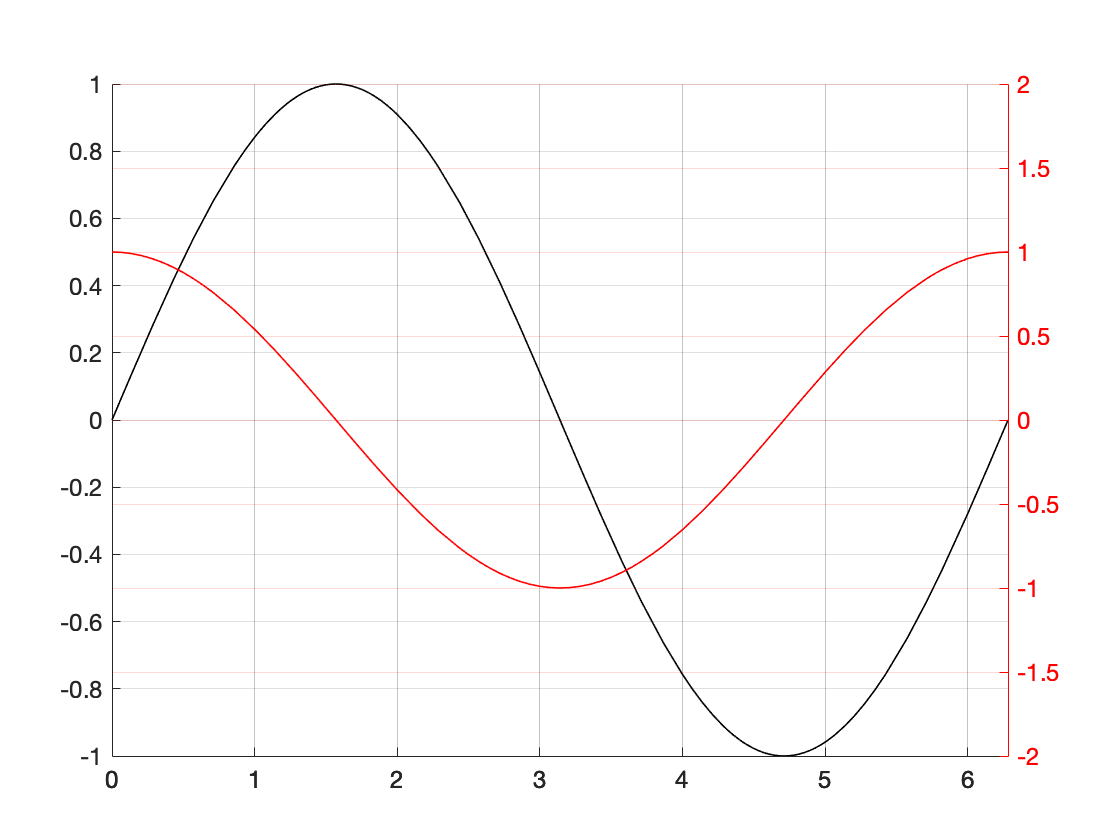
\includegraphics[width=8cm]{/Users/guilhermesalome/Teaching/Duke/Econ890 Matlab - 2019/supporting/matlab_manipulating_axes.png}
\caption{\label{fig:orgdd93b42}
Manipulating Axes to Generate a Figure with Two y-Axis.}
\end{figure}

We can manipulate the axes to create complex figures.
An example, is creating a figure with multiple y-axes.
\lstset{language=matlab,label= ,caption= ,captionpos=b,firstnumber=1,numbers=left,style=Matlab-editor}
\begin{lstlisting}
% create figure window
fig = figure;
% add two overlapping axes
ax1 = axes(fig, 'Position', [0.1 0.1 0.8 0.8], ...
           'XLim', [0, 2*pi], 'YLim', [-1, 1]);
ax2 = axes(fig, 'Position', [0.1 0.1 0.8 0.8], ...
           'XLim', [0, 2*pi], 'YLim', [-1, 1]);
% create one plot per axes
p1 = fplot(ax1, @sin, [0, 2*pi]);
p2 = fplot(ax2, @cos, [0, 2*pi]);

% remove the color of both axes, so that both plots can be
% displayed no matter the order we add the plots
ax2.Color = 'none';
ax1.Color = 'none';
% add color to the background of the figure
fig.Color = 'white';

% both plots use a y-axis and both are on the left of the figure
% and are overlapping
% let's move the y-axis of the 2nd plot to the right of the figure
ax2.YAxisLocation = 'right';

% change the y-limits of the second axes
ax2.YLim = [-2, 2];

% notice that we have two sets of tick marks on both sides
% this happens because the ax1 marks extend to the side of ax2
% and the same happen with the ax2 marks extending to the side ax1
% we can remove these by setting the Box property to off
ax1.Box = 'off';                        % removes marks on right side
ax2.Box = 'off';                        % removes marks on left side

% we can add grids to the figure
% however, the grids use the tick marks from one of the y-axis
% we can choose which axes to use with the axes command
% choose the first axes
axes(ax1);
grid on;
% it is also possible to add another grid using the tick marks
% using the 2nd y-axis
% choose the second axes
axes(ax2);
grid on;

% change the color of the second y-axis
ax2.YColor = [1 0 0];
% change the color of  the line to match the axis
p2.Color = ax2.YColor;
\end{lstlisting}
We can use the above to create all sorts of figures.
All we have to keep in mind is that a \texttt{figure window} is a blank canvas, to which we add axes.
The axes can be created in various positions and moved around.
Lastly, we add the actual plots to these axes.
\section{Summary}
\label{sec:orgfcd2119}
We have covered some of the plotting capabilities of Matlab.
You should be able to:
\begin{itemize}
\item Create histograms with \texttt{histogram}
\item Create scatter plots with \texttt{scatter} and modify the size and color of the marks using data
\item Add labels (\texttt{xlabel} and \texttt{ylabel}), legends (\texttt{legend}) and a title (\texttt{title}) to plots
\item Add a color bar (\texttt{colorbar}) and a grid (\texttt{grid}) to plots
\item Store a figure with the \texttt{.fig} format using \texttt{savefig} and then load it with \texttt{openfig}
\item Save a figure to the \texttt{.png} format and specifying its resolution with \texttt{print}
\item Create 2-D line plots with \texttt{plot} and change the size, color and style of the line
\item Modify the range of the x-axis and y-axis with \texttt{xlim} and \texttt{ylim}
\item Use Latex in figures
\item Add text to the figure with \texttt{text}
\item Create surface plots with \texttt{surf}
\item Generate data for surface plots with \texttt{meshgrid}
\item Quickly plot functions with \texttt{fplot}
\item Change the tick marks and the labels with \texttt{xticks} and \texttt{xticklabels}
\item Create figures with multiple subplots using \texttt{subplot}
\item Set default property values for plots with \texttt{set} and \texttt{groot}
\item Understand the building blocks of figures: \texttt{figure} and \texttt{axes}
\item Create more complicated figures by creating and manipulating axes
\item Create overlapping figures
\item Create plots with two y-axes
\end{itemize}
\section{Assignment}
\label{sec:orgdecee32}
There are many other types of plots we have not covered, like the ones generated with the functions \href{https://www.mathworks.com/help/matlab/ref/bar.html?s\_tid=doc\_ta}{\texttt{bar}} and \href{https://www.mathworks.com/help/matlab/ref/contour.html?s\_tid=doc\_ta}{\texttt{contour}}.
We will cover some other important tools for plotting in the assignment problems.
However, a full documentation of the plotting facilities in Matlab is available on the \href{https://www.mathworks.com/help/matlab/2-and-3d-plots.html}{2-D and 3-D plots} reference page.

\begin{problem}
Use the housing data set to estimate a linear regression of the logarithm of the median house value on the logarithm of the total number of bedrooms.
Given the beta estimate, compute \(\E{\ln{\text{Median House Value}}\vert\ln{\text{Total Bedrooms}}}\) over a range of values for the total number of bedrooms (say from \(1\) to \(30\)) and make a plot with the values.
\end{problem}

\begin{problem}
Using the standard error estimates for \(\hat{\beta}\), create a \(95\%\) confidence interval \(\E{\ln{\text{Median House Value}}\vert\ln{\text{Total Bedrooms}}}\).
Extend the plot from the previous problem with the confidence interval.
\end{problem}

\begin{problem}
(Shading Confidence Intervals)
Use the functions \href{https://www.mathworks.com/help/matlab/ref/fill.html?s\_tid=doc\_ta}{\texttt{fill}} and \href{https://www.mathworks.com/help/matlab/ref/flip.html?s\_tid=doc\_ta}{\texttt{flip}} to shade the area between the confidence interval.
The function \texttt{fill} colors an area defined by connecting points, from start to finish.
To create these points you can use the function \texttt{flip}.
\end{problem}

\begin{problem}
When we call the function \texttt{fill}, it returns a \texttt{Patch} object.
There are two properties of the \texttt{Patch} object that we can use to improve the shading of the confidence interval.
The properties are the \texttt{LineStyle} and the \texttt{FaceAlpha}.
Set the \texttt{LineStyle} property value to \texttt{'none'}.
What does this property do?
Set the \texttt{FaceAlpha} property value to \texttt{0.2}.
What does this property do?
\end{problem}

\begin{problem}
Download the following file: \href{https://github.com/matlab-for-economists/data}{\texttt{AAPL.csv}}.
The file follows the \href{https://en.wikipedia.org/wiki/Comma-separated\_values}{.csv} format and contains the stock price of the publicly traded company \href{https://en.wikipedia.org/wiki/Apple\_Inc.}{Apple Inc.}
The file has 3 columns (no headers): date, time and price.
The first column contains the date of a given price in the \texttt{YYYYMMDD} format.
For example, a date of \texttt{20070103} means January 3rd of 2007.
The second column contains the time of a given price in the \texttt{HHMM} format.
For example, a time of \texttt{935} means that the price in the 3rd column was recorded at 9:35 am.
The last column contains the stock price in dollars at the given date and time.

Load the data into Matlab.
There are various functions for importing data into Matlab, choose the \href{https://www.mathworks.com/help/matlab/import\_export/supported-file-formats.html}{appropriate function}.
\end{problem}

\begin{problem}
The geometric return of a stock over a time interval that starts at time \(t-1\) and ends at time \(t\) is given by:
\begin{align*}
r_t \equiv \ln{\frac{P_t}{P_{t-1}}}
\end{align*}
where \(P_t\) is the price of the stock at time \(t\).

The stock market is open only during some hours of the day, closing at around 4 pm.
The data you downloaded has prices sampled every 5-minutes of the day.
We can use this data to compute intraday returns and overnight returns.
Intraday returns are returns of a stock within a day.
In this case, we can compute intraday returns for every 5 minutes interval.
Overnight returns are the returns from the time the market closes at a given day, to the time the market opens on the next day.

Compute the \uline{intraday} geometric returns from the stock prices.
You should use the function \href{https://www.mathworks.com/help/matlab/ref/reshape.html?s\_tid=doc\_ta}{\texttt{reshape}} to facilitate the computation of the intraday returns.
\end{problem}

\begin{problem}
Create a histogram of the intraday geometric returns.
\end{problem}

\begin{problem}
(Optional) Read about \href{https://en.wikipedia.org/wiki/Kernel\_density\_estimation}{Kernel density estimation}.
Use the function \href{https://www.mathworks.com/help/stats/ksdensity.html?s\_tid=doc\_ta}{\texttt{ksdensity}} to estimate the density of the distribution of the intraday returns.
\end{problem}

\begin{problem}
Create a 2D-line plot of the intraday returns.
For the x-axis use a range of numbers, say \texttt{1:length(returns)}.
\end{problem}

\begin{problem}
To modify the x-axis so that it correctly displays timestamps, we need to use the first two columns of the data set to obtain serial date numbers.
This format is used by Matlab to display timestamps in time series plots.
Use the function \href{https://www.mathworks.com/help/matlab/ref/datenum.html}{\texttt{datenum}} to convert the first two columns of data set into the serial date format.
Specifically, use the syntax \texttt{datenum(Y, M, D, H, MN)} to obtain the serial dates.
\end{problem}

\begin{problem}
Plot the time series of intraday returns.
Now, use the serial dates for the x-axis.
After the \texttt{plot} command, you can use the function \href{https://www.mathworks.com/help/matlab/ref/datetick.html?s\_tid=doc\_ta}{\texttt{datetick}} to automatically change the tick labels to the appropriate value.
For example, if you want to show tick labels for years, you would execute \texttt{datetick('x', 'yyyy')}.
\end{problem}

\begin{problem}
We can use Matlab to generate animations from plots.
Adapt \href{https://www.mathworks.com/help/matlab/creating\_plots/line-animation-of-streaming-data.html}{this example} to display an animation of the evolution of prices over time.
You can do this by creating an \href{https://www.mathworks.com/help/matlab/ref/animatedline.html?s\_tid=doc\_ta}{\texttt{animatedline}} object.
Then, specify the \href{https://www.mathworks.com/help/matlab/ref/axis.html?s\_tid=doc\_ta\#buk989s-1-limits}{\texttt{axis}} limits, so that it is not updated every time we draw new points to the figure.
Then, \href{https://www.mathworks.com/help/matlab/ref/addpoints.html?s\_tid=doc\_ta}{\texttt{addpoints}} to the plot and draw them with the command \href{https://www.mathworks.com/help/matlab/ref/drawnow.html?s\_tid=doc\_ta}{\texttt{drawnow}}.
You should add the points and draw them in a for-loop.
The speed of the animation is controlled by how many points you loop through.

If you want to save this animation into a file (you do not need to do it for this exercise), you should read the \href{https://www.mathworks.com/help/matlab/ref/imwrite.html\#btv452g-1}{Write Animated GIF} example.
\end{problem}
\newpage
\printbibliography
\newpage
\end{document}